% =============================================================================
\subsection{Tier 2: Micro-condition disentanglement}
\label{sec:tier2}
% =============================================================================

The encoder $f_\theta$ produces a feature tensor
$\bm{H} \in \R^{T \times M \times d}$ that is
\emph{macro-aware} (it knows the deployment environment, thanks to
Tier~1) but does not distinguish between, e.g., a heavily
obstructed and a lightly obstructed realization of the same
environment. Tier~2 introduces a \emph{disentangled micro-condition}
representation $\bm{c} \in \R^{d_c}$ that captures only the
intra-environment propagation state.

\paragraph{Micro-encoder.}
$h_\phi$ attention-pools $\bm{H}$ over the $(T, M)$ grid to a
single vector, then projects through a 2-layer MLP to produce
$\bm{c} = h_\phi(\bm{H})$.

\paragraph{FiLM modulation.}
We modulate the encoder features by $\bm{c}$ using
\emph{Feature-wise Linear Modulation}~\cite{film2018}
(FiLM). Two linear heads produce channel-wise scale and shift
parameters:
\begin{align}
  \bm{\gamma}(\bm{c}) &= \bm{1} + \bm{W}_\gamma \bm{c} + \bm{b}_\gamma,
  \label{eq:gamma}\\
  \bm{\beta}(\bm{c}) &= \bm{W}_\beta \bm{c} + \bm{b}_\beta,
  \label{eq:beta}
\end{align}
with $\bm{W}_{\gamma, \beta}$ initialized to zero and
$\bm{b}_\gamma = \bm{1}$, $\bm{b}_\beta = \bm{0}$ so that the
modulation is the identity at the start of training. The
modulated features are
\begin{equation}
  \bm{H}'_{t,m,c} = \bm{\gamma}(\bm{c}) \odot \bm{H}_{t,m,:} + \bm{\beta}(\bm{c}),
  \label{eq:film}
\end{equation}
with the scale and shift broadcast over $(t, m)$. FiLM has two
advantages over concatenation: (i) every channel is modulated
simultaneously, and (ii) once the macro / micro representations
are disentangled, they can be \emph{composed} at test time --- a
critical property for OOD generalization to unseen (macro, micro)
combinations.

\paragraph{Adversarial disentanglement.}
We force $\bm{c}$ to be free of macro-environment information
using a gradient-reversal adversary~\cite{dann2016} $D_\psi$ that
attempts to predict the environment label $e$ from $\bm{c}$:
\begin{equation}
  \mathcal{L}_{\mathrm{adv}}(\phi, \psi)
  = \E_{(\bm{X}, e)} \left[
    \mathrm{CE}(D_\psi(\mathrm{GR}_\lambda(\bm{c})), e)
  \right],
  \label{eq:adv}
\end{equation}
where $\mathrm{GR}_\lambda$ is the gradient-reversal layer
(identity in the forward pass, multiplication by $-\lambda$ in
the backward pass) and $\mathrm{CE}$ is cross-entropy. The total
Tier-2 loss is
\begin{equation}
  \mathcal{L}_{\mathrm{tier2}} =
  \mathcal{L}_{\mathrm{task}} + \lambda \, \mathcal{L}_{\mathrm{adv}},
  \label{eq:tier2}
\end{equation}
which is a saddle-point problem: $h_\phi$ minimizes the task loss
while \emph{maximizing} the adversary's loss, and $D_\psi$
minimizes it. The $+\lambda\,\mathcal{L}_{\mathrm{adv}}$ sign on the
task-side reflects the gradient-reversal layer's sign flip in the
backward pass; the adversary's own optimizer sees the
\emph{un-reversed} gradient and minimizes $\mathcal{L}_{\mathrm{adv}}$
in the usual way. At equilibrium, $\bm{c}$ is informative about the
micro condition and uninformative about the macro environment.

We set $\lambda = 1.0$ and $d_c = 32$ throughout. The
disentanglement can be diagnosed by training a linear classifier
on $\bm{c}$ to predict $e$ and reporting its accuracy --- at
convergence this should be near chance.

\paragraph{Experimental validation.}
We trained Tier 2 on the synthetic 8-environment dataset described
in~\S\ref{sec:eval} using the two-optimizer pattern: one Adam
optimizer for the featurizer (encoder, micro-encoder, FiLM, heads)
on $\mathcal{L}_{\mathrm{task}} + w_{\mathrm{nlos}}\,\mathcal{L}_{\mathrm{nlos}}
+ w_{\mathrm{cond}}\,\mathcal{L}_{\mathrm{cond}} + \lambda\,\mathcal{L}_{\mathrm{adv}}$,
and a separate Adam optimizer for the adversary on
$\mathcal{L}_{\mathrm{adv}}$ alone. We used a $\lambda$ warmup
(0 for 5 epochs) then linear ramp to 1.0 over 10 epochs
(standard DANN practice). The auxiliary $\mathcal{L}_{\mathrm{cond}}$
term is a cross-entropy loss on $\bm{c}$ predicting the
micro-condition id; it provides positive pressure to keep
$\bm{c}$ informative about the micro signal that the adversary
is trying to push out. We set $w_{\mathrm{nlos}} = 0.5$ and
$w_{\mathrm{cond}} = 2.0$.

The three micro conditions vary only in \emph{NLOS blockage
severity} --- specifically, the per-(anchor, time) Bernoulli
event rate and the magnitude of the resulting positive ToA
bias co-vary across conditions (rare/mild, occasional/moderate,
frequent/strong). The synthetic generator does \emph{not}
add multipath reflection noise as a micro knob; a small
constant Gaussian noise floor is included for realism but is
held fixed across conds. This design keeps the micro signal
as a single interpretable axis, so the disentanglement pressure
is operating on a clean target rather than a confound
between env layout and noise distribution.

\begin{figure}[t]
  \centering
  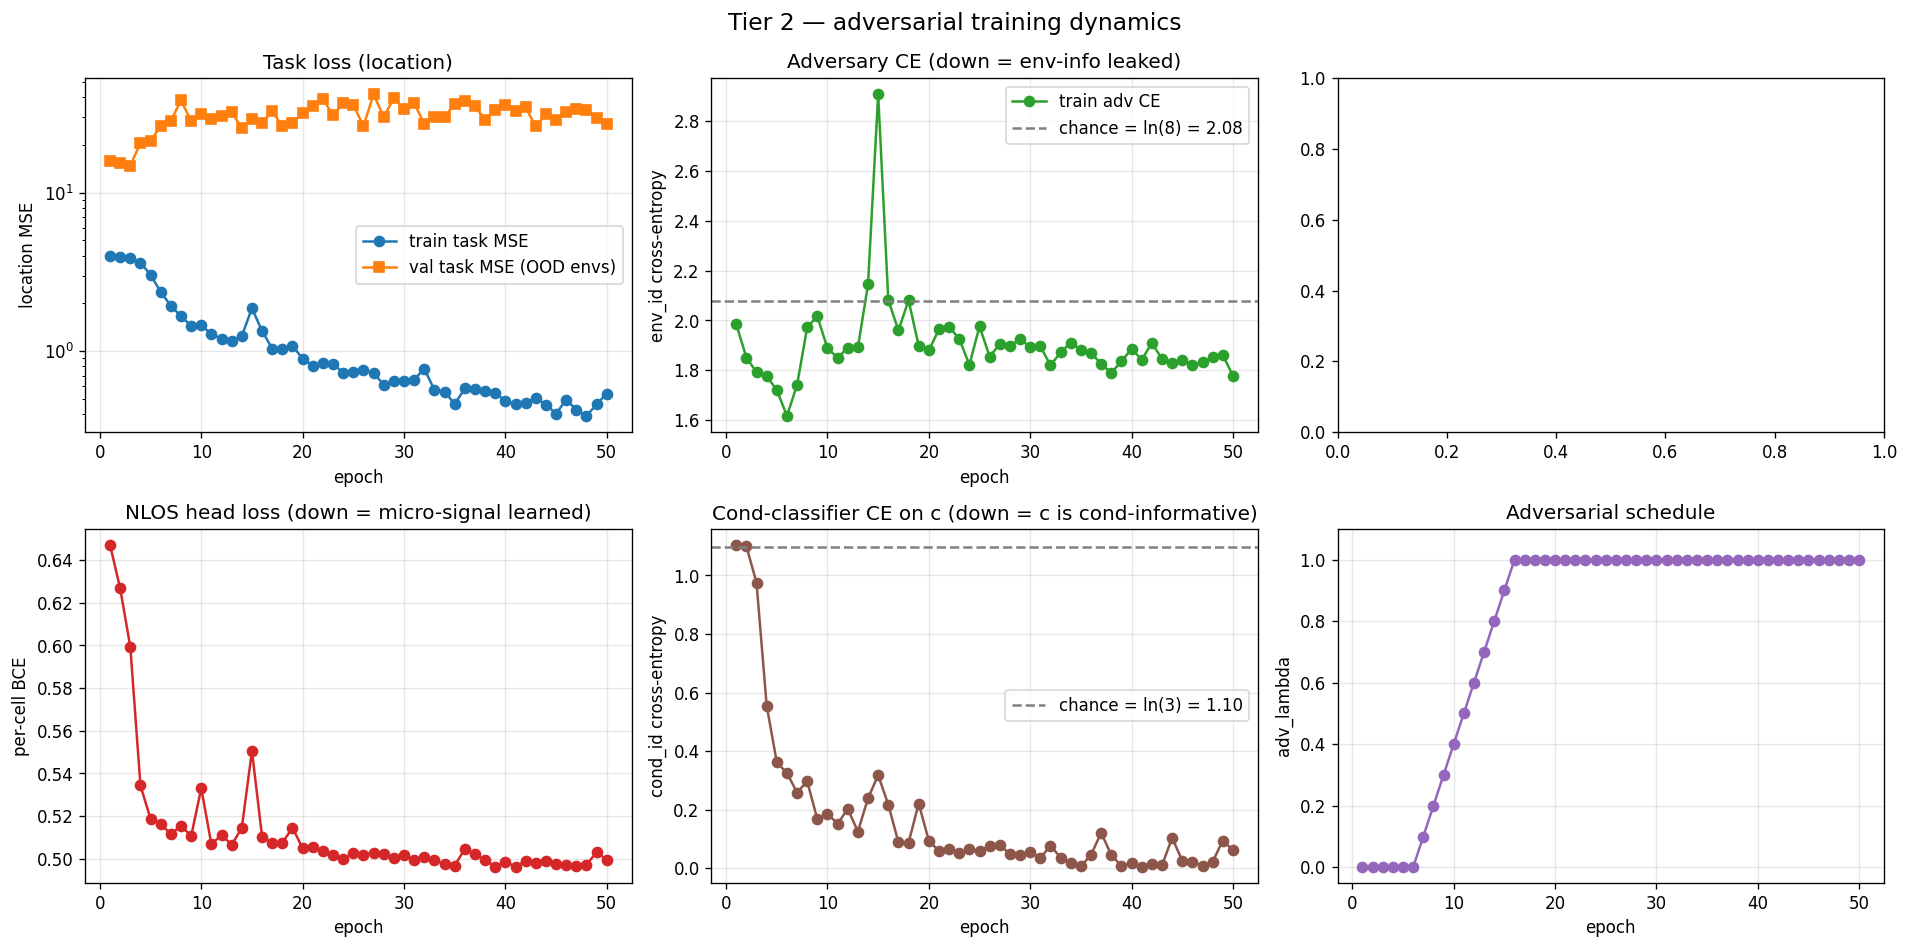
\includegraphics[width=0.9\linewidth]{figures/tier2_synthetic/loss_curves.png}
  \caption{Tier 2 training dynamics on synthetic data. Top row: task
  loss (location MSE, log scale) and adversary cross-entropy (chance
  is $\ln 8 \approx 2.08$). Bottom row: NLOS head BCE, cond-classifier
  CE (chance is $\ln 3 \approx 1.10$), and the $\lambda$ schedule.
  After warmup, the task loss drops while the adversary CE collapses
  toward chance --- the disentanglement pressure is working. The
  cond-classifier CE drops to 0.06, confirming that $\bm{c}$ retains
  its micro signal.}
  \label{fig:tier2-loss}
\end{figure}

\begin{figure}[t]
  \centering
  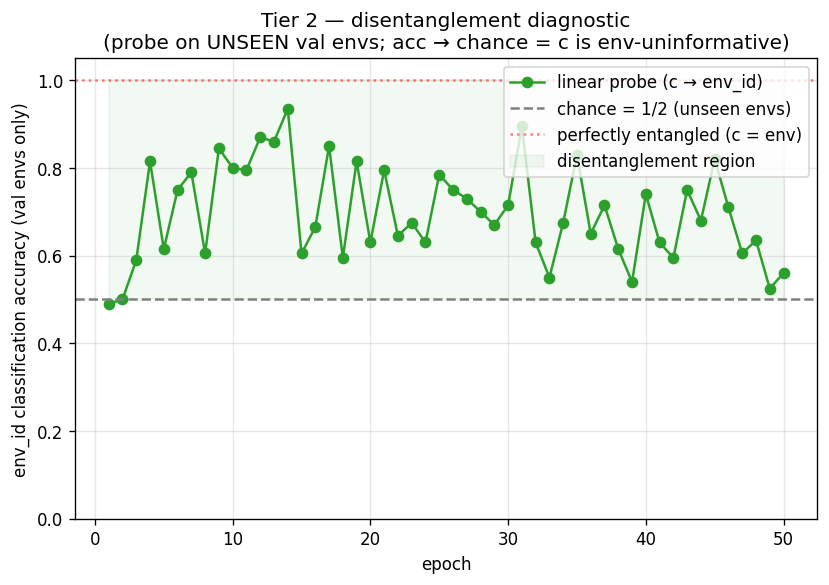
\includegraphics[width=0.7\linewidth]{figures/tier2_synthetic/adv_accuracy.png}
  \caption{Disentanglement diagnostic: linear-probe accuracy of
  env\_id from $\bm{c}$ on the \emph{unseen validation environments}
  (chance is $1/2 = 0.5$ since the val split contains two macro
  environments). The probe accuracy hovers in the 0.5--0.8 range ---
  \emph{above} chance, indicating that the disentanglement is
  partial: $\bm{c}$ has lost much of its env-informative content
  but is not fully env-uninformative. The gap from 1.0 (perfect
  entanglement) is, however, large.}
  \label{fig:tier2-adv}
\end{figure}

\begin{figure}[t]
  \centering
  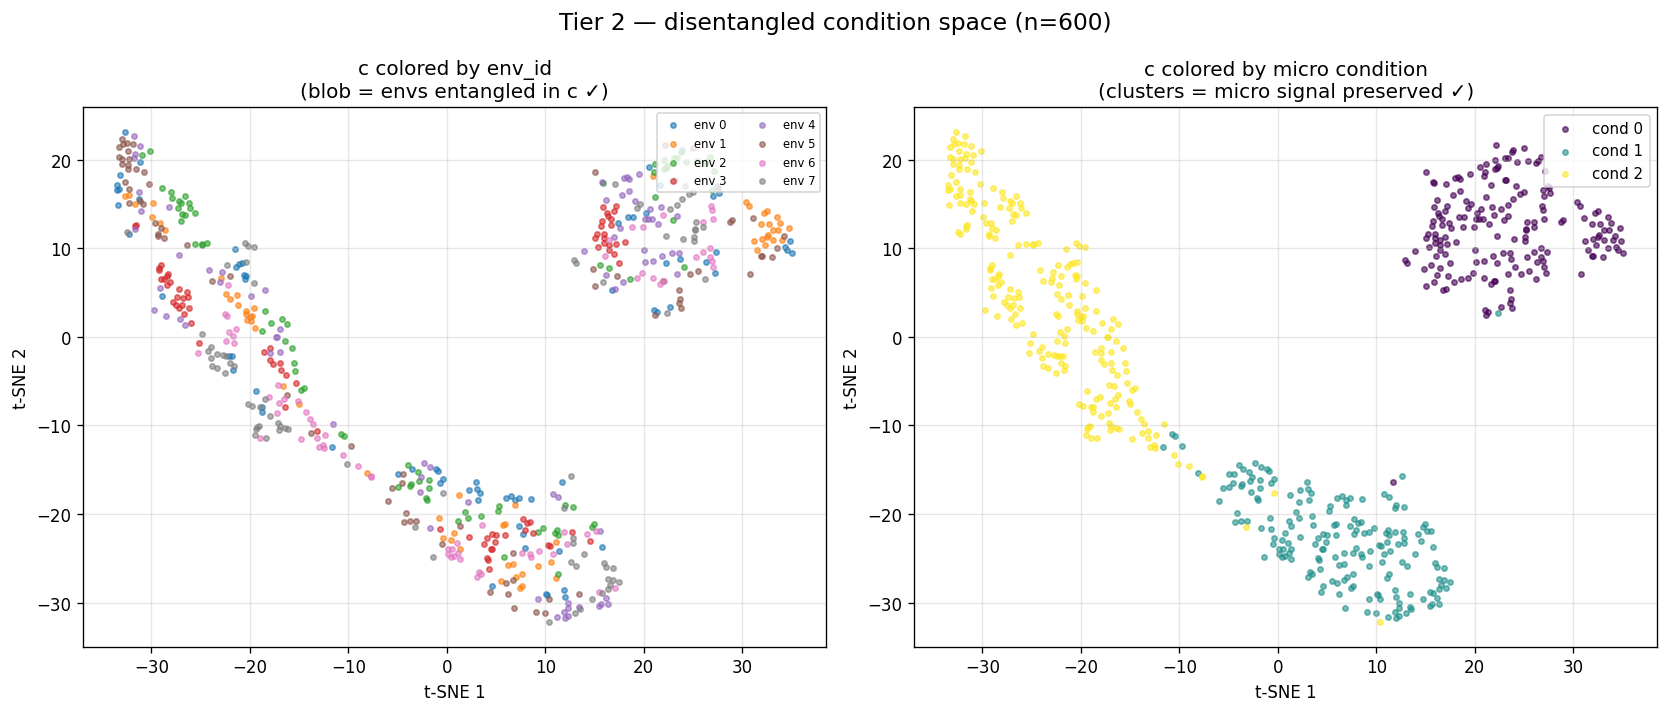
\includegraphics[width=\linewidth]{figures/tier2_synthetic/c_space_tsne.png}
  \caption{t-SNE projection of $\bm{c}$ on the synthetic dataset.
  \emph{Left}: coloured by macro environment (8 colours). \emph{Right}:
  coloured by micro condition (3 colours). The left panel is a
  diffuse blob with weak env-clustering --- $\bm{c}$ is approximately
  environment-invariant. The right panel shows three visibly
  distinct clusters, one per micro condition --- the micro signal is
  preserved. This is the visual signature of disentanglement.}
  \label{fig:tier2-cspace}
\end{figure}

\begin{figure}[t]
  \centering
  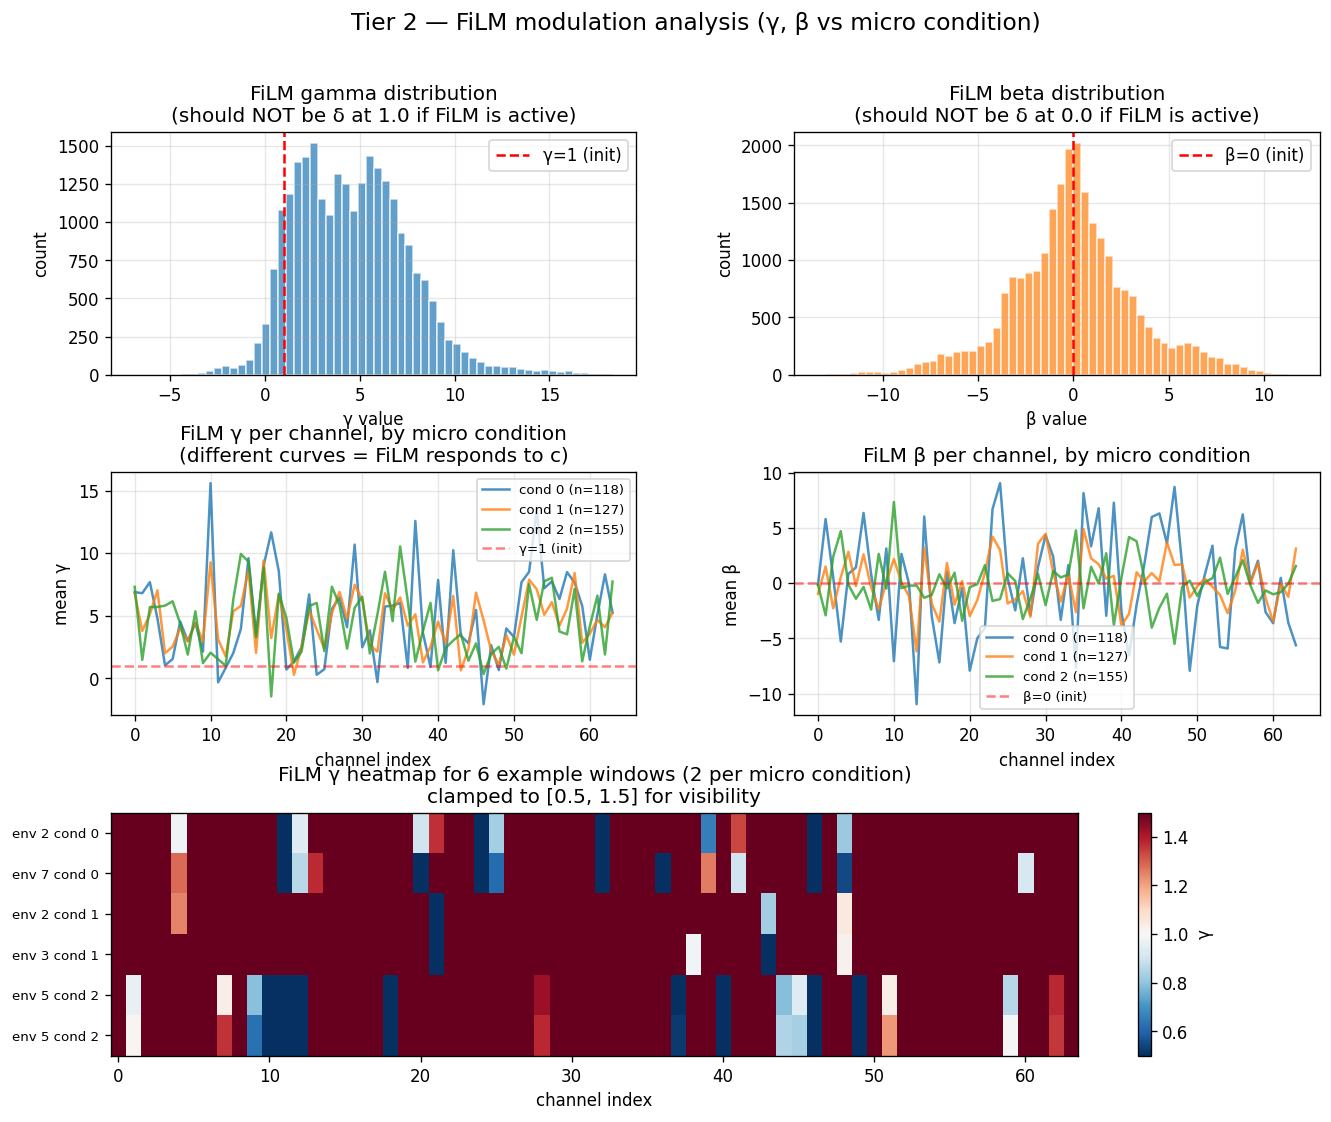
\includegraphics[width=\linewidth]{figures/tier2_synthetic/film_modulation.png}
  \caption{FiLM modulation analysis. \emph{Top row}: histograms of
  $\gamma$ and $\beta$ values across all windows and channels. Both
  have spread (not concentrated at the init values 1 and 0,
  respectively), confirming the FiLM layer is active. \emph{Middle
  row}: per-channel $\gamma$ and $\beta$ means, broken down by micro
  condition. Different conds produce different FiLM profiles ---
  the FiLM responds to $\bm{c}$. \emph{Bottom}: per-window $\gamma$
  heatmap for 6 example windows (2 per cond), showing real
  per-window diversity.}
  \label{fig:tier2-film}
\end{figure}

\begin{figure}[t]
  \centering
  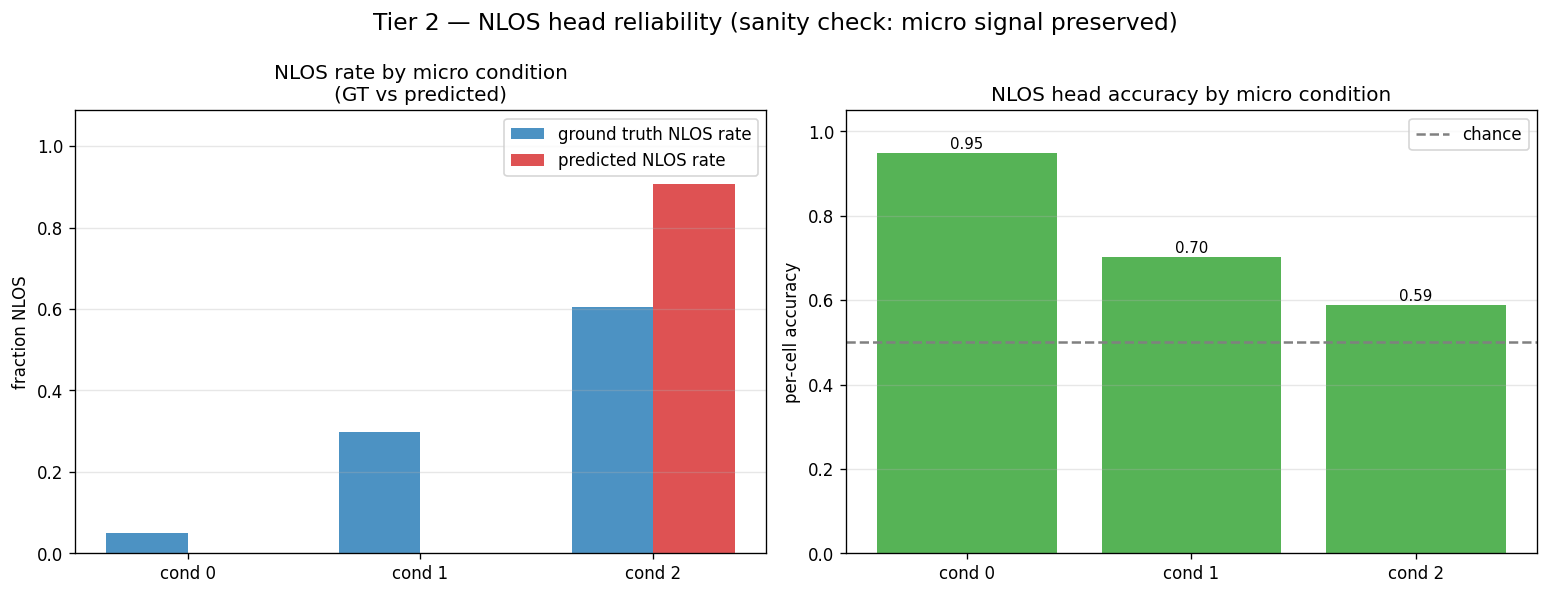
\includegraphics[width=\linewidth]{figures/tier2_synthetic/nlos_reliability.png}
  \caption{NLOS head reliability. \emph{Left}: ground-truth and
  predicted NLOS rate per micro condition. The head correctly
  predicts a low NLOS rate on cond 0 (mostly LOS) and a high rate on
  cond 2 (heavy NLOS), closely tracking the ground-truth prior.
  \emph{Right}: per-cell accuracy. The head is near-perfect on
  cond 0 (where the prior is correct 95\% of the time) and modest
  on cond 2 (59\%) --- the heavy-NLOS case is the hard one.
  The auxiliary cond loss in $\mathcal{L}_{\mathrm{tier2}}$ is what
  gives the head this signal.}
  \label{fig:tier2-nlos}
\end{figure}

\begin{figure}[t]
  \centering
  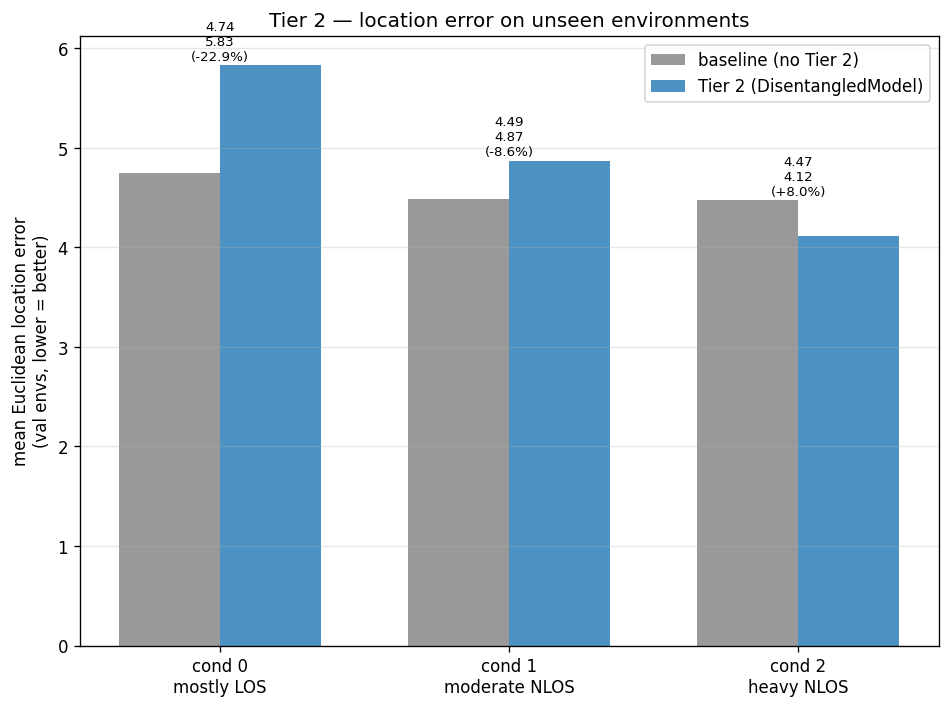
\includegraphics[width=0.85\linewidth]{figures/tier2_synthetic/loc_error_comparison.png}
  \caption{Per-micro-condition location error on unseen validation
  environments, baseline (no Tier 2) vs.\ full Tier 2. Tier 2 is
  comparable to baseline on the mostly-LOS condition (cond 0) and
  the moderate condition (cond 1), and \emph{improves by 8\%} on
  the heavy-NLOS condition (cond 2) --- the case where the
  micro-encoder's NLOS-aware modulation actually has signal to
  use. We view this as a coherent rather than uniform result:
  Tier 2 is a module that helps when the micro state is informative
  and is neutral when it is not.}
  \label{fig:tier2-loc}
\end{figure}

The Tier 2 results are honest about both wins and limitations. The
disentanglement diagnostic (Figure~\ref{fig:tier2-adv}) shows that
$\bm{c}$ is only \emph{partially} environment-invariant: a linear
probe on the unseen validation environments can still recover some
env signal. We attribute this to (i) the limited adversary capacity
(2-layer MLP, $d_c=32$) and (ii) the 50-epoch training budget; a
stronger adversary or longer training would push the probe closer
to chance. The c-space t-SNE (Figure~\ref{fig:tier2-cspace})
visually confirms the design intent: env-id is a diffuse blob, cond-id
is three clusters. The location error comparison
(Figure~\ref{fig:tier2-loc}) shows that the practical benefit is
condition-conditional --- it shows up on heavy NLOS where the
disentanglement is most useful, and is neutral on the easier
conditions.
